\documentclass[12pt, letterpaper]{article}

% ==========================================
%              DOCUMENT PACKAGES
% ==========================================

% --- Core Language & Encoding ---
\usepackage[english]{babel} % Sets the language and regional settings for English documents
\usepackage[utf8]{inputenc} % Allows the use of UTF-8 characters in the document
\usepackage[T1]{fontenc} % Specifies the font encoding
\usepackage[margin=1.5cm]{geometry} % Sets the page margins

% --- Colors & Graphics ---
\usepackage[table,dvipsnames]{xcolor} % Advanced color management
% \usepackage{color} % Basic package for text and background colors
\usepackage{graphicx} % Enhanced support for including external images and scaling them
\usepackage{adjustbox} % Adjusts the size, scaling, and alignment of boxes, images, and tables
% \usepackage{background} % Allows adding background images or watermarks to pages
\usepackage{float} % Improves the interface for floating objects and adds the [H] placement
\usepackage{pdflscape} % Makes landscape pages display correctly on screen in PDF viewers
\usepackage{pdfpages} % Allows the inclusion of external multi-page PDF documents

% --- Math, Science & Engineering ---
\usepackage{amsfonts} % Provides extended mathematical fonts
\usepackage{amsmath} % Provides advanced mathematical typesetting and environments
\usepackage{amssymb} % Provides extended mathematical symbols
% \usepackage{amsmath, amssymb} % (Redundant combination line omitted for stability)
\usepackage{amsthm} % Facilitates the creation of theorem-like environments
\usepackage{mathtools} % Enhances amsmath with additional math tools and bug fixes
\usepackage{thmtools} % Extensions and customization options for theorem environments
\usepackage{nicematrix} % Enhances matrices and tabulars using PGF/TikZ
\usepackage{xy} % Typesets complex graphs and diagrams
\usepackage{circuitikz} % Allows drawing of electrical networks and circuits

% --- Typography & Fonts ---
\usepackage{avant} % Sets the default sans-serif font to Avant Garde
\usepackage{cantarell} % Sets the default sans-serif font to Cantarell
\usepackage{charter} % Sets the default roman font to Charter
\usepackage{cmbright} % Sets the font family to Computer Modern Bright 
\usepackage{helvet} % Sets the default sans-serif font to Helvetica
\usepackage{inconsolata} % Sets the default typewriter (monospace) font to Inconsolata
\usepackage{iwona} % Sets the font family to Iwona 
\usepackage{kurier} % Sets the font family to Kurier 
\usepackage{lmodern} % Loads the Latin Modern fonts 
\usepackage{textcomp} % Provides additional text symbols
\usepackage{ulem} % Provides various types of text underlining and strikethroughs

% --- Tables & Lists ---
\usepackage{array} % Extends the array and tabular environments
\usepackage{arydshln} % Allows dashed lines in arrays and tables
\usepackage{bigstrut} % Adds custom vertical space in table rows
\usepackage{booktabs} % Enhances the quality of tables with better horizontal rules
% \usepackage{colortbl} % Allows coloring of rows, columns, and individual cells in tables
\usepackage{diagbox} % Creates table cells with diagonal lines 
\usepackage{enumitem} % Provides advanced control over list environments
\usepackage{longtable} % Allows tables to break across multiple pages
\usepackage{multirow} % Allows individual table cells to span across multiple rows
\usepackage{tabularx} % Creates tables with dynamically adjustable-width columns
\usepackage{pgfplotstable} % Reads and cleanly formats numerical tables directly from CSV

% --- Formatting, Layout & UI ---
\usepackage{blindtext} % Generates dummy text for testing document layouts
\usepackage{caption} % Customizes captions in floating environments
\usepackage{comment} % Allows you to block out large sections of text
\usepackage{emptypage} % Automatically removes headers and footers on empty pages
\usepackage{fancyhdr} % Allows complete customization of headers and footers
\usepackage{fancyvrb} % Enhanced verbatim environments for writing raw code
\usepackage{framed} % Creates framed, shaded, or differently highlighted text regions
\usepackage{fullpage} % Quickly sets all page margins to 1 inch
\usepackage{lipsum} % Generates Lorem Ipsum dummy text
\usepackage{mdframed} % Creates highly customizable framed environments
\usepackage{multicol} % Allows intermixing single and multiple text columns
\usepackage{parskip} % Replaces standard paragraph indentation with vertical spacing
\usepackage{setspace} % Controls line spacing (single, one-and-a-half, double)
\usepackage{subcaption} % Supports sub-figures and sub-tables with independent captions
% \usepackage{subfig} % Older package for sub-figures (subcaption is generally preferred now)
\usepackage{tcolorbox} % Creates heavily customized colored and framed text boxes
\usepackage{titlesec} % Customizes the formatting of section, subsection, and chapter headings
\usepackage{titling} % Provides advanced control over the typesetting of the document title

% --- Bibliographies & References ---
\usepackage{biblatex} % Advanced, modern bibliographic processing and formatting
\usepackage{csquotes} % Context-sensitive quotation facilities
\usepackage{makeidx} % Supports the generation of a document index
% \usepackage{natbib} % Flexible bibliography support, particularly for author-year citation styles

% --- TikZ & Plotting ---
\usepackage{tikz} % Advanced package for creating vector graphics and diagrams programmatically
\usepackage{pgf-pie} % Draws pie charts programmatically using PGF/TikZ
\usepackage{pgfplots} % Creates high-quality mathematical plots, charts, and graphs
% \usepackage{fancytikzposter} % Used to create large format academic posters using TikZ

% --- URLs & Hyperlinks ---
\usepackage{url} % Formats and properly hyphenates long URLs
\usepackage{breakurl} % Allows line breaks in URLs, especially when compiled with latex -> dvips
\usepackage{hyperref} % Creates cross-referencing, clickable links, and PDF bookmarks

% --- Code Formatting ---
\usepackage{listings} % Typesets programming source code with formatting and syntax highlighting


% ==========================================
%           DOCUMENT CONFIGURATION
% ==========================================

% Custom color definitions
\definecolor{mygray}{gray}{0.9}

% Hyperlink configuration
\hypersetup{
    colorlinks=true,
    linkcolor=blue,
    urlcolor=blue
}

% Configuración adicional para breaks en URLs
\def\UrlBreaks{\do\/\do-\do_\do.\do=\do?\do\&}
\expandafter\def\expandafter\UrlBreaks\expandafter{\UrlBreaks\do\a\do\b\do\c\do\d\do\e\do\f\do\g\do\h\do\i\do\j\do\k\do\l\do\m\do\n\do\o\do\p\do\q\do\r\do\s\do\t\do\u\do\v\do\w\do\x\do\y\do\z}

%Uncomment the following lines to use a sans-serif font
\renewcommand{\familydefault}{\sfdefault}

% TikZ libraries
\usetikzlibrary{shapes.geometric, positioning, decorations.pathreplacing}

\graphicspath{ {./img/} } % Sets the path for the graphics

\newlist{biblio}{enumerate}{1}
\setlist[biblio,1]{label=[\arabic*]}

\makeindex

% \tiny
% \scriptsize
% \footnotesize
% \small
% \normalsize (default size)
% \large
% \Large
% \LARGE
% \huge
% \Huge


% ==========================================
%         GLOBAL LISTINGS SETTINGS
% ==========================================
\lstset{
	basicstyle=\ttfamily\small,
	numbers=left,
	numberstyle=\tiny\color{gray},
	stepnumber=1,
	numbersep=10pt,
	backgroundcolor=\color{white},
	showspaces=false,
	showstringspaces=false,
	breaklines=true,
	frame=single,
	tabsize=2, 
    captionpos=b, 
    lineskip=-1pt,
	extendedchars=true,
	literate={á}{{\'a}}1 {é}{{\'e}}1 {í}{{\'i}}1 {ó}{{\'o}}1 {ú}{{\'u}}1 {Á}{{\'A}}1 {É}{{\'E}}1 {Í}{{\'I}}1 {Ó}{{\'O}}1 {Ú}{{\'U}}1 {ñ}{{\~n}}1 {Ñ}{{\~N}}1 {¿}{{\textquestiondown}}1 {¡}{{\textexclamdown}}1
}

% ==========================================
%            LANGUAGE: SQL
% ==========================================
\lstdefinestyle{sqlstyle}{
	language=SQL,
	keywordstyle=\color{blue}\bfseries,
	commentstyle=\color[rgb]{0,0.5,0}\itshape,
	stringstyle=\color{red}
}

% ==========================================
%            LANGUAGE: VHDL
% ==========================================
\lstdefinelanguage{VHDL}{
	morekeywords={entity, architecture, signal, port, in, out, inout, begin, end, process, if, then, else, elsif, case, when, others, for, while, loop, wait, library, use, std_logic, std_logic_vector, integer, boolean, rising_edge, falling_edge, component, generic, map, downto, to, and, or, not, xor, nand, nor, xnor},
	morecomment=[l]{--},
	morestring=[b]",
	sensitive=false,
	alsoletter={_}
}

\lstdefinestyle{vhdl}{
	language=VHDL,
	keywordstyle=\color{blue}\bfseries,
	commentstyle=\color[rgb]{0,0.6,0}\itshape,
	stringstyle=\color{red}
}

% ==========================================
%              LANGUAGE: C
% ==========================================
\lstdefinestyle{cstyle}{
	language=C,
	keywordstyle=\color{blue}\bfseries,
	commentstyle=\color[rgb]{0,0.5,0}\itshape,
	stringstyle=\color{red},
	directivestyle=\color{purple},
    tabsize=4 % Overrides the global tabsize of 2 for C code specifically
}

% ==========================================
%             LANGUAGE: C++
% ==========================================
\lstdefinestyle{cppstyle}{
	language=C++,
	keywordstyle=\color{blue}\bfseries,
	commentstyle=\color[rgb]{0,0.5,0}\itshape,
	stringstyle=\color{red},
	directivestyle=\color{purple},
    tabsize=4
}

% ==========================================
%           LANGUAGE: PYTHON
% ==========================================
\lstdefinestyle{pythonstyle}{
	language=Python,
	keywordstyle=\color{blue}\bfseries,
	commentstyle=\color[rgb]{0,0.5,0}\itshape,
	stringstyle=\color{red},
    % Python relies heavily on indentation, so keeping tabsize aligned is important
    tabsize=4
}

% ==========================================
%             LANGUAGE: BASH
% ==========================================
\lstdefinestyle{bashstyle}{
	language=bash,
	keywordstyle=\color{blue}\bfseries,
	commentstyle=\color[rgb]{0,0.5,0}\itshape,
	stringstyle=\color{red},
    % Bash variables often use $, so we can highlight them dynamically if needed
    moredelim=[s][\color{orange}]{\$\{}{\}}
}

% ==========================================
%           LANGUAGE: ASSEMBLY
% ==========================================
\lstdefinestyle{asmstyle}{
	language=[x86masm]Assembler,
	keywordstyle=\color{blue}\bfseries,
	commentstyle=\color[rgb]{0,0.5,0}\itshape,
	stringstyle=\color{red},
    % Adding common ARM/Microcontroller instructions for better highlighting
    morekeywords={ldr, str, mov, cmp, add, sub, b, bl, bx, push, pop, svc, eor, and, orr, lsl, lsr}
}

% % Configure header
\setlength{\headheight}{28pt} % Adjust header height for two-line header
\pagestyle{fancy}
\fancyhf{} % Clear all header and footer fields
\lhead{\textbf{Nombre:} Ugartechea González Luis Antonio -- 320223822 \\ \textbf{Asignatura:} <asignatura>, \textbf{Grupo:} <grupo>}
\renewcommand{\headrulewidth}{0.4pt}

\begin{document}

\newgeometry{margin=1.5cm}
\begin{titlepage}
    \noindent
    \renewcommand{\arraystretch}{1.5}
    % Definimos la tabla principal con dos columnas exactamente iguales (50/50)
    \begin{tabularx}{\textwidth}{|>{\centering\arraybackslash}X|>{\centering\arraybackslash}X|}
        \hline
        % Fila superior: Combinamos las dos columnas e insertamos una sub-tabla
        \multicolumn{2}{|@{}c@{}|}{%
            \begin{tabularx}{\dimexpr\textwidth-2\arrayrulewidth\relax}{m{3.5cm}|>{\centering\arraybackslash}X}
                \centering \vspace{0.2cm} 
\includegraphics[width=2cm,height=2.5cm]{escudoFI_color.png} & \large \textbf{Fundamentos de Sistemas Embebidos}
            \end{tabularx}%
        } \\
        \hline
        % Fila inferior: Alineada a la mitad exacta
        \large Facultad de Ingeniería & \large UNAM \\
        \hline
    \end{tabularx}

    \vspace{0.5cm}

    \begin{center}
        {\fontsize{35}{48}\selectfont Laboratorio de Fundamentos de} \\
        {\fontsize{35}{48}\selectfont Sistemas Embebidos\par}
        % Línea divisoria azul (se puede ajustar el tono de azul)
        \textcolor{MidnightBlue!70}{\rule{\textwidth}{1pt}}
    \end{center}

    \vspace{2cm}

    \begin{center}
        % Aumenta el espaciado entre filas para que coincida con el formato
        % \renewcommand{\arraystretch}{1.8}
        \fontsize{15}{21}\selectfont
        % Columna 1: Alineada a la derecha, en cursiva (itshape) y de 4.5cm de ancho
        % Columna 2: Alineada a la izquierda
        \begin{tabular}{>{\raggedleft\arraybackslash\itshape}p{4.5cm} @{\hspace{0.5cm}} l}
            Profesor(a): & \underline{\makebox[10cm][l]{ Eduardo Fragoso Navarro}} \\
            Asignatura: & \underline{\makebox[10cm][l]{ Fundamentos de Sistemas Embebidos}} \\
            Grupo: & \underline{\makebox[10cm][l]{3}} \\
            No de Práctica(s): & \underline{\makebox[10cm][l]{8}} \\
            Integrante(s): & \underline{\makebox[10cm][l]{Tepal Briseño Hansel Yael - 320078282}} \\
            & \underline{\makebox[10cm][l]{Ugartechea González Luis Antonio - 320223822}} \\
            No. de brigada: & \underline{\makebox[10cm][l]{12}} \\
            Semestre: & \underline{\makebox[10cm][l]{ 9\(^\circ\)}} \\
            Fecha de entrega: & \underline{\makebox[10cm][l]{3 de noviembre de 2026}} \\
            Observaciones: & \underline{\makebox[10cm][l]{}} \\
            & \underline{\makebox[10cm][l]{}} \\
        \end{tabular}
    \end{center}

\end{titlepage}
\restoregeometry

\newpage
\fontsize{25}{21}\selectfont CALIFICACIÓN: \underline{\makebox[10cm][l]{}}
\newpage
\normalsize

\section*{\centering \fontsize{14}{17}\sffamily\selectfont Node-RED: control de un programa de Python por SSH}

\section*{\centering \fontsize{14}{17}\sffamily\selectfont Objetivo}

El objetivo principal de esta práctica consiste en instalar e implementar Node-RED mediante un contenedor de Docker dentro de una placa Orange Pi Zero 2W, explorando las ventajas del paradigma de la programación low-code orientada a dispositivos IoT. A través de esta plataforma, se busca establecer una interfaz de control visual basada en flujos que permita gestionar la ejecución de procesos en el hardware, facilitando el prototipado rápido sin la necesidad de programar toda la lógica de integración de manera manual.

De manera específica, se pretende diseñar un flujo capaz de arrancar, detener y consultar el estado de un script de Python (\texttt{2\_puntos.py}), el cual está encargado de generar gráficos en movimiento dentro de una pantalla ILI9341 conectada a la placa. Para lograr el control de este proceso, el contenedor de Node-RED establecerá una conexión segura hacia la placa a través de SSH mediante el uso de llaves públicas y privadas, ejecutando comandos remotos de systemd para modificar el estado del servicio del programa de forma automatizada.

\section*{\centering \fontsize{14}{17}\sffamily\selectfont Resultados y Anaĺisis}

\subsection*{Ejercicio 1: Instalar Node-RED con Docker}

En el primer ejercicio se llevó a cabo la instalación y despliegue de Node-RED utilizando un contenedor de Docker en la Orange Pi Zero 2W. Como resultado, se logró levantar el contenedor exitosamente en segundo plano y se comprobó su estado activo mediante el comando \texttt{docker ps}. A continuación, se muestra la salida de la terminal confirmando que el contenedor \texttt{nodered} se encuentra en ejecución:

% \lstinputlisting[
%     style=bashstyle,
%     caption={Comprobación del contenedor de Node-RED}
% ]{evidence/docker.txt}

\begin{figure}[H]
    \centering
    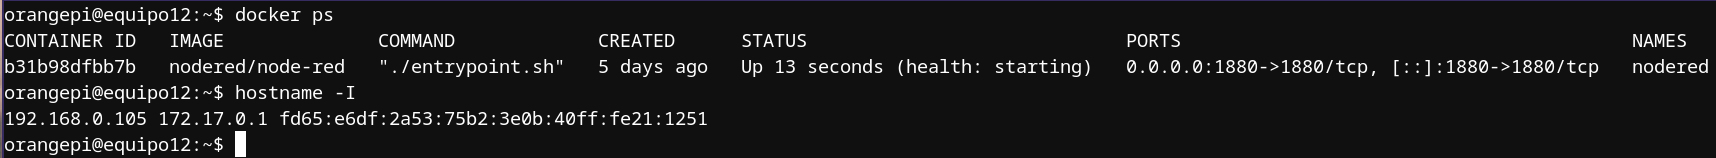
\includegraphics[width=\textwidth]{nodered_active.png}
    \caption{Salida de la terminal mostrando el contenedor de Node-RED en ejecución.}
    \label{fig:nodered_docker}
\end{figure}

\begin{figure}[H]
    \centering
    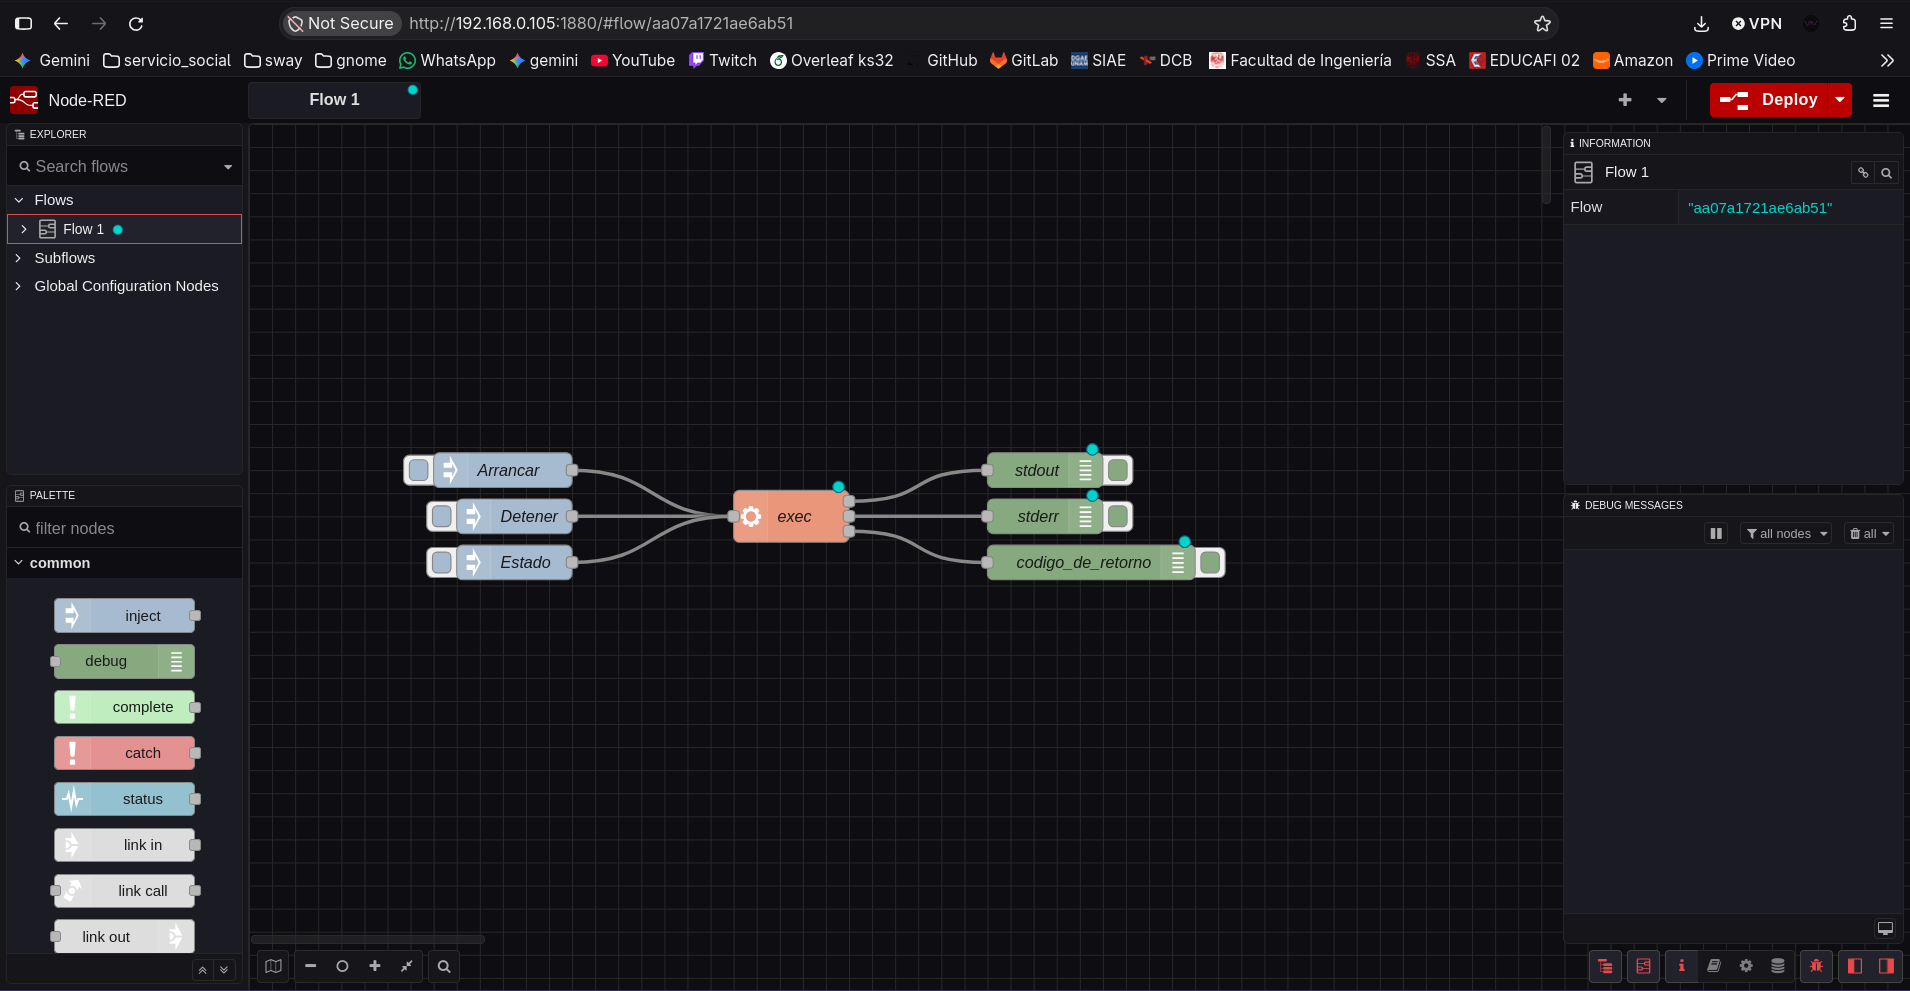
\includegraphics[width=\textwidth]{nodered_app.png}
    \caption{Interfaz web de Node-RED accesible desde el navegador de la PC.}
    \label{fig:nodered_web}
\end{figure}

Es importante mencionar la configuración de la carpeta persistente montada como volumen a través del parámetro \texttt{-v "\$PWD/data":/data}. Dado que los contenedores son momentáneos por naturaleza, este mapeo hacia el sistema de archivos de la placa garantiza que toda la información crítica de Node-RED —tales como los flujos de trabajo diseñados y las futuras llaves SSH— no se pierda al detener o eliminar el contenedor. Asimismo, la asignación de permisos adecuados para el usuario \texttt{uid 1000} (correspondiente al usuario \texttt{orangepi}) resultó indispensable para evitar errores de escritura al momento en que el contenedor intentara guardar datos en el directorio local de la placa. Finalmente, el mapeo de puertos (\texttt{-p 1880:1880}) fue lo que permitió exponer la aplicación aislada hacia la red local, habilitando su control externo.

\subsection*{Ejercicio 2: Dejar listo el servicio puntos}

En el segundo ejercicio se preparó el servicio \texttt{puntos} para que su ejecución sea controlada exclusivamente por Node-RED, evitando que arranque de manera automática al encender la placa. Para lograr esto, se deshabilitó y detuvo el servicio utilizando los comandos \texttt{systemctl --user disable puntos} y \texttt{systemctl --user stop puntos}. Posteriormente, se verificó su estado para confirmar que el proceso se encontrara inactivo.

A continuación, se muestra la salida en la terminal comprobando que el servicio fue detenido correctamente:

\begin{figure}[H]
    \centering
    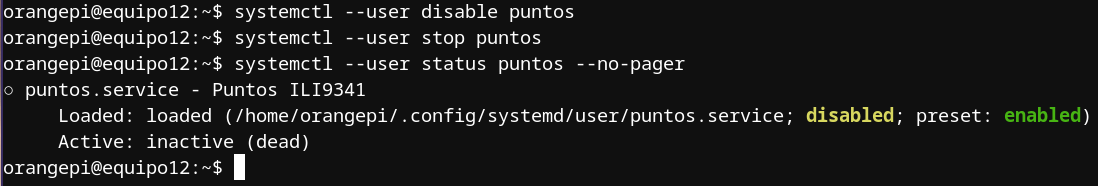
\includegraphics[width=\textwidth]{servicio_puntos.png}
    \caption{Salida de la terminal mostrando el servicio \texttt{puntos} detenido.}
    \label{fig:servicio_puntos_detenido}
\end{figure}

Una vez garantizado que el servicio no iniciaba por sí solo, se realizó una prueba manual arrancando y deteniendo el servicio (\texttt{systemctl --user start puntos} y \texttt{systemctl --user stop puntos}) para comprobar que el hardware respondía correctaser evide mente antes de involucrar a Node-RED.

\begin{figure}[h!]
    \centering
    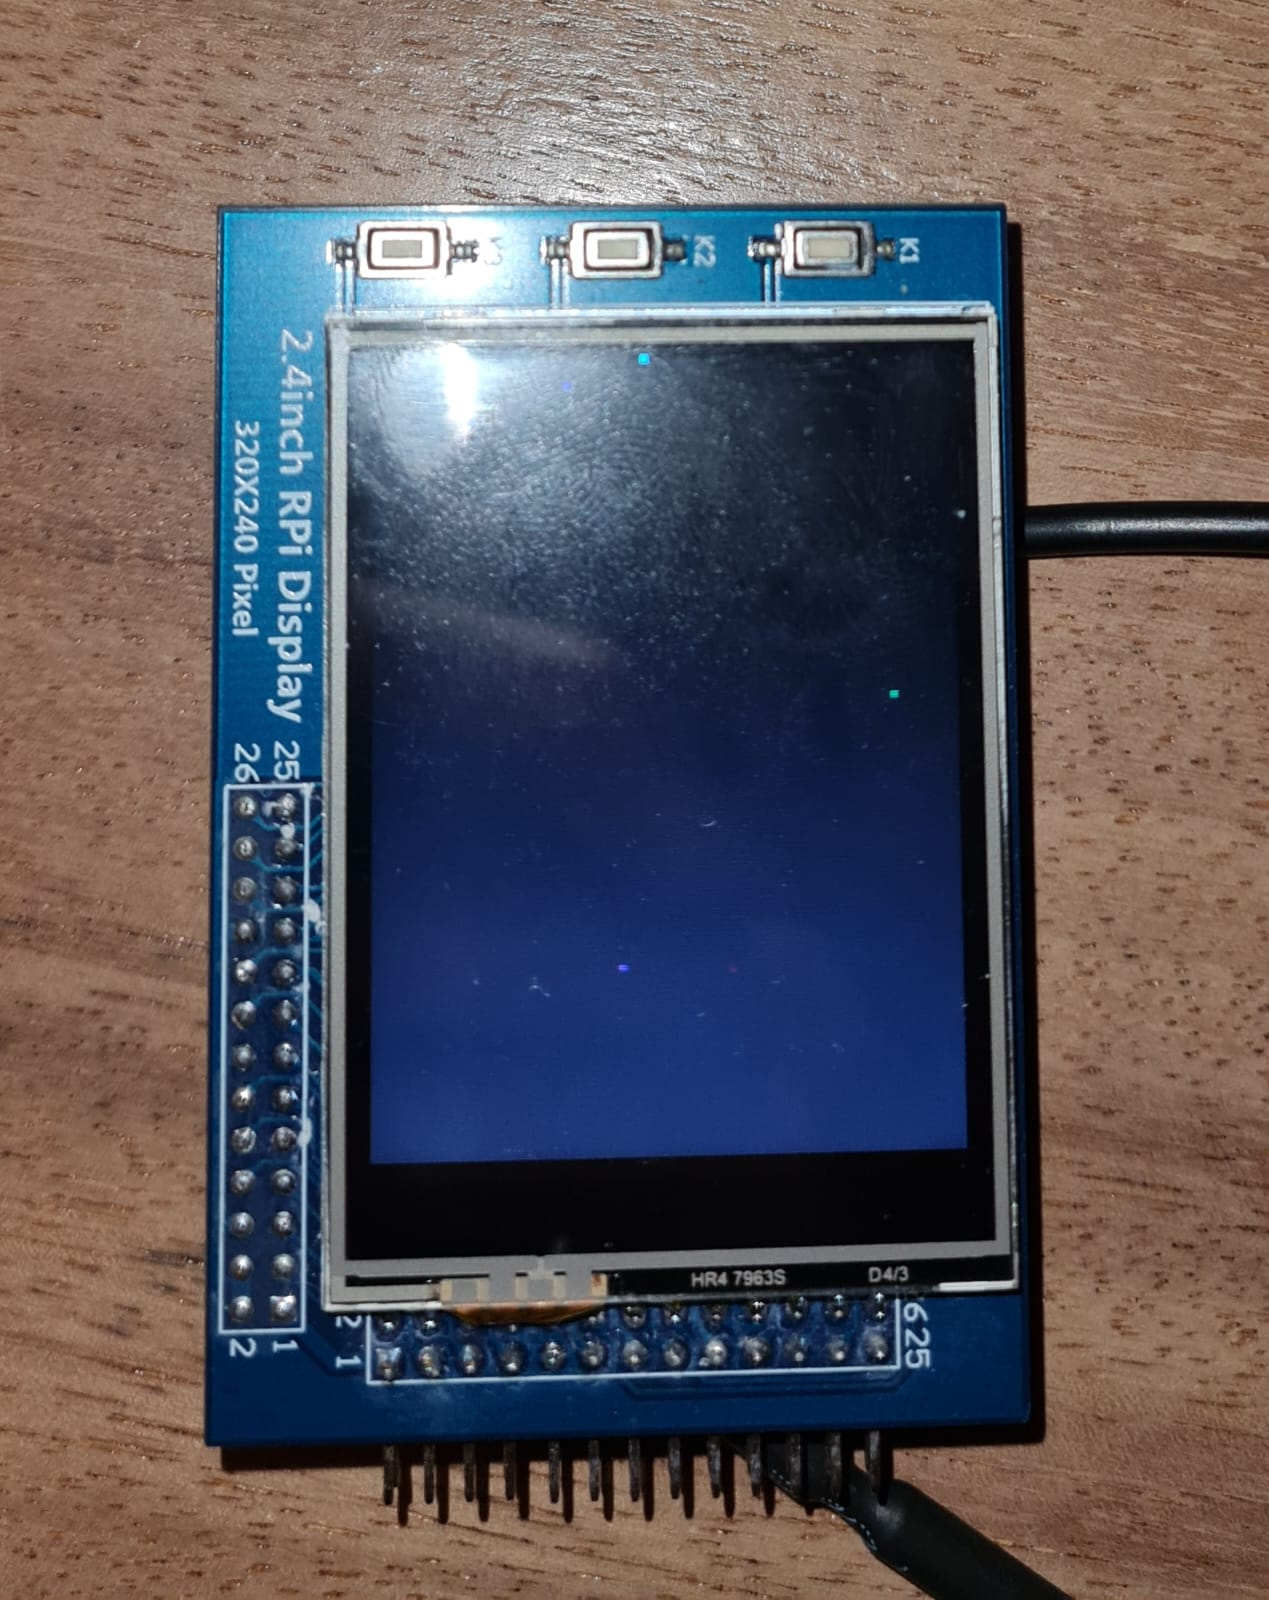
\includegraphics[width=0.45\textwidth]{puntos_1.jpeg}
    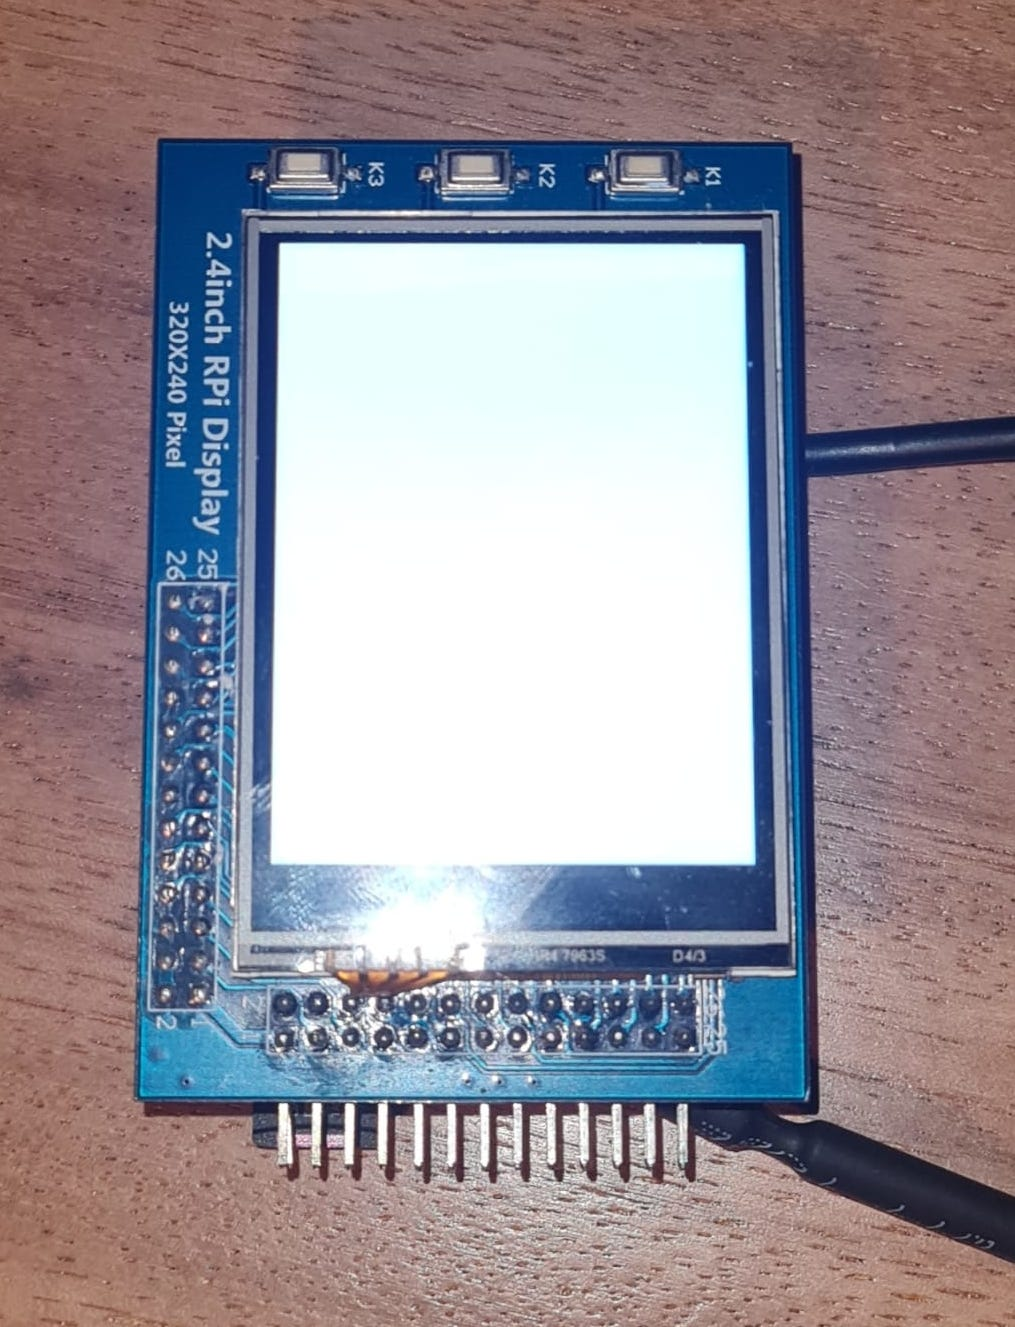
\includegraphics[width=0.45\textwidth]{puntos_2.jpeg}
    \caption{Prueba del servicio mostrando los puntos en la pantalla física ILI9341.}
    \label{fig:prueba_pantalla}
\end{figure}

Aquí notamos la importancia de aislar las capas de control en el desarrollo con sistemas embebidos. Al evitar que el programa inicie con el sistema operativo, se previenen bloqueos de acceso al hardware, de lo contrario, si Node-RED intentara iniciar un proceso que ya está usando la pantalla, se generaría un error de colisión de recursos (\textit{Device or resource busy}) debido a que la interfaz no soporta múltiples programas escribiendo simultáneamente. Además, realizar la prueba manual de \texttt{systemd} actúa como un punto de control fundamental: permite validar que el script de Python y el bus de datos hacia la pantalla funcionan correctamente por sí solos. De esta forma, si ocurren fallos en los siguientes ejercicios, el diagnóstico será más sencillo al saber que el problema radicaría en la conexión SSH o en la lógica del flujo, y no en la ejecución local del programa.

\subsection*{Ejercicio 3: SSH sin contraseña desde el contenedor}

En el tercer ejercicio, se configuró y verificó el acceso remoto mediante SSH sin contraseña desde el interior del contenedor de Node-RED hacia el sistema operativo de la placa. Dado que las llaves criptográficas (pública y privada) ya habían sido generadas previamente dentro de la carpeta persistente y la llave pública ya constaba en el archivo \texttt{\textasciitilde{}/.ssh/authorized\_keys} del usuario anfitrión, la actividad se centró en comprobar la persistencia de esta configuración y validar la comunicación.

Para confirmar que el enlace seguro seguía habilitado, se ejecutó un comando de prueba desde el contenedor solicitando a la placa que imprimiera un mensaje, obteniendo una respuesta exitosa sin que el sistema solicitara credenciales interactivas:

\begin{figure}[H]
    \centering
    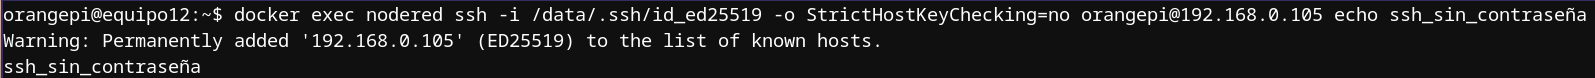
\includegraphics[width=\textwidth]{ssh_key.png}
    \caption{Prueba de conexión SSH desde el contenedor hacia la placa.}
    \label{fig:sshtest}
\end{figure}

Posteriormente, se comprobó que, a través de esta misma conexión SSH, el contenedor contaba con los privilegios necesarios para interactuar con el administrador de servicios \texttt{systemd} del usuario en la placa base, enviando una consulta remota sobre el estado del servicio de los puntos:

\begin{figure}[H]
    \centering
    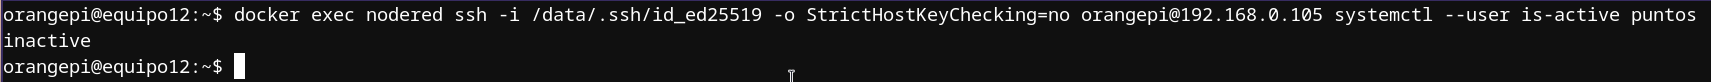
\includegraphics[width=\textwidth]{service_status.png}
    \caption{Prueba de control remoto de \texttt{systemd} desde el contenedor.}
    \label{fig:sshsystemctl}
\end{figure}

Se observa la eficiencia de combinar volúmenes de Docker con autenticación asimétrica. Al tener la llave privada alojada en el directorio montado \texttt{/data/.ssh}, la identidad del contenedor sobrevive a reinicios, permitiendo la automatización sostenida. Asimismo, el uso de los parámetros \texttt{-i} (para apuntar a la ruta exacta de la llave privada) y \texttt{-o StrictHostKeyChecking=no} resulta vital para este tipo de arquitecturas IoT; puesto que Node-RED opera en segundo plano como un servicio desatendido, carece de una terminal interactiva para aceptar huellas criptográficas (\textit{fingerprints}) de nuevos dispositivos o para teclear contraseñas. Esta delegación de permisos confirma que Node-RED puede solicitar acciones en el hardware subyacente manteniendo las barreras de seguridad del contenedor intactas.

\subsection*{Ejercicio 4: El flujo en Node-RED}

En el último ejercicio se comprobó el funcionamiento del sistema utilizando la interfaz gráfica de Node-RED. Dado que la configuración de los nodos (tres nodos \texttt{inject}, un nodo \texttt{exec} y tres nodos \texttt{debug}) y la conexión SSH ya estaban establecidas, el objetivo fue validar que los comandos enviados desde la interfaz web lograran arrancar, detener y consultar el estado del servicio \texttt{puntos} de manera efectiva.

Al desplegar (\textit{Deploy}) el flujo y abrir el panel de mensajes (\textit{debug}) en Node-RED, se procedió a interactuar con los nodos \texttt{inject}. Primero, se comprobó el estado inactivo del servicio presionando el inyector correspondiente, lo cual generó un mensaje \texttt{"inactive\textbackslash{}n"} en la salida estándar (debug 1) y un código de error normal en la salida de retorno (debug 3), confirmando que \texttt{systemd} reconocía el servicio pero este no estaba corriendo.

A continuación, se presenta el diagrama completo del flujo implementado en Node-RED:

\begin{figure}[H]
    \centering
    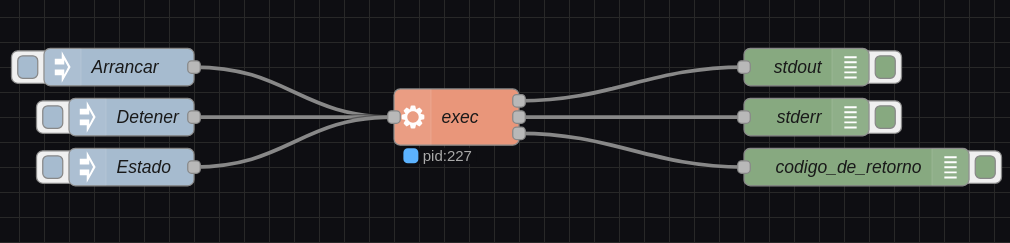
\includegraphics[width=\textwidth]{flujo_nodered.png}
    \caption{Diagrama del flujo en Node-RED para el control del servicio \texttt{puntos}.}
    \label{fig:flujo_nodered}
\end{figure}

Posteriormente, se inyectó el comando de arranque (\texttt{start puntos}). Esto se reflejó inmediatamente en la ejecución del script en la placa, donde los gráficos comenzaron a renderizarse de manera fluida en la pantalla ILI9341. El panel de depuración mostró un código de retorno \texttt{0} en debug 3, indicando una ejecución remota exitosa sin errores en stderr (debug 2). Al volver a consultar el estado, la salida cambió exitosamente a \texttt{active}. Finalmente, se activó el inyector de detención (\texttt{stop puntos}), logrando detener la animación instantáneamente, comprobando así el control bidireccional asíncrono entre el entorno \textit{low-code} y el \textit{hardware} embebido.

Para respaldar el análisis, se capturó la salida del panel debug durante las transiciones de estado:

\begin{figure}[H]
    \centering
    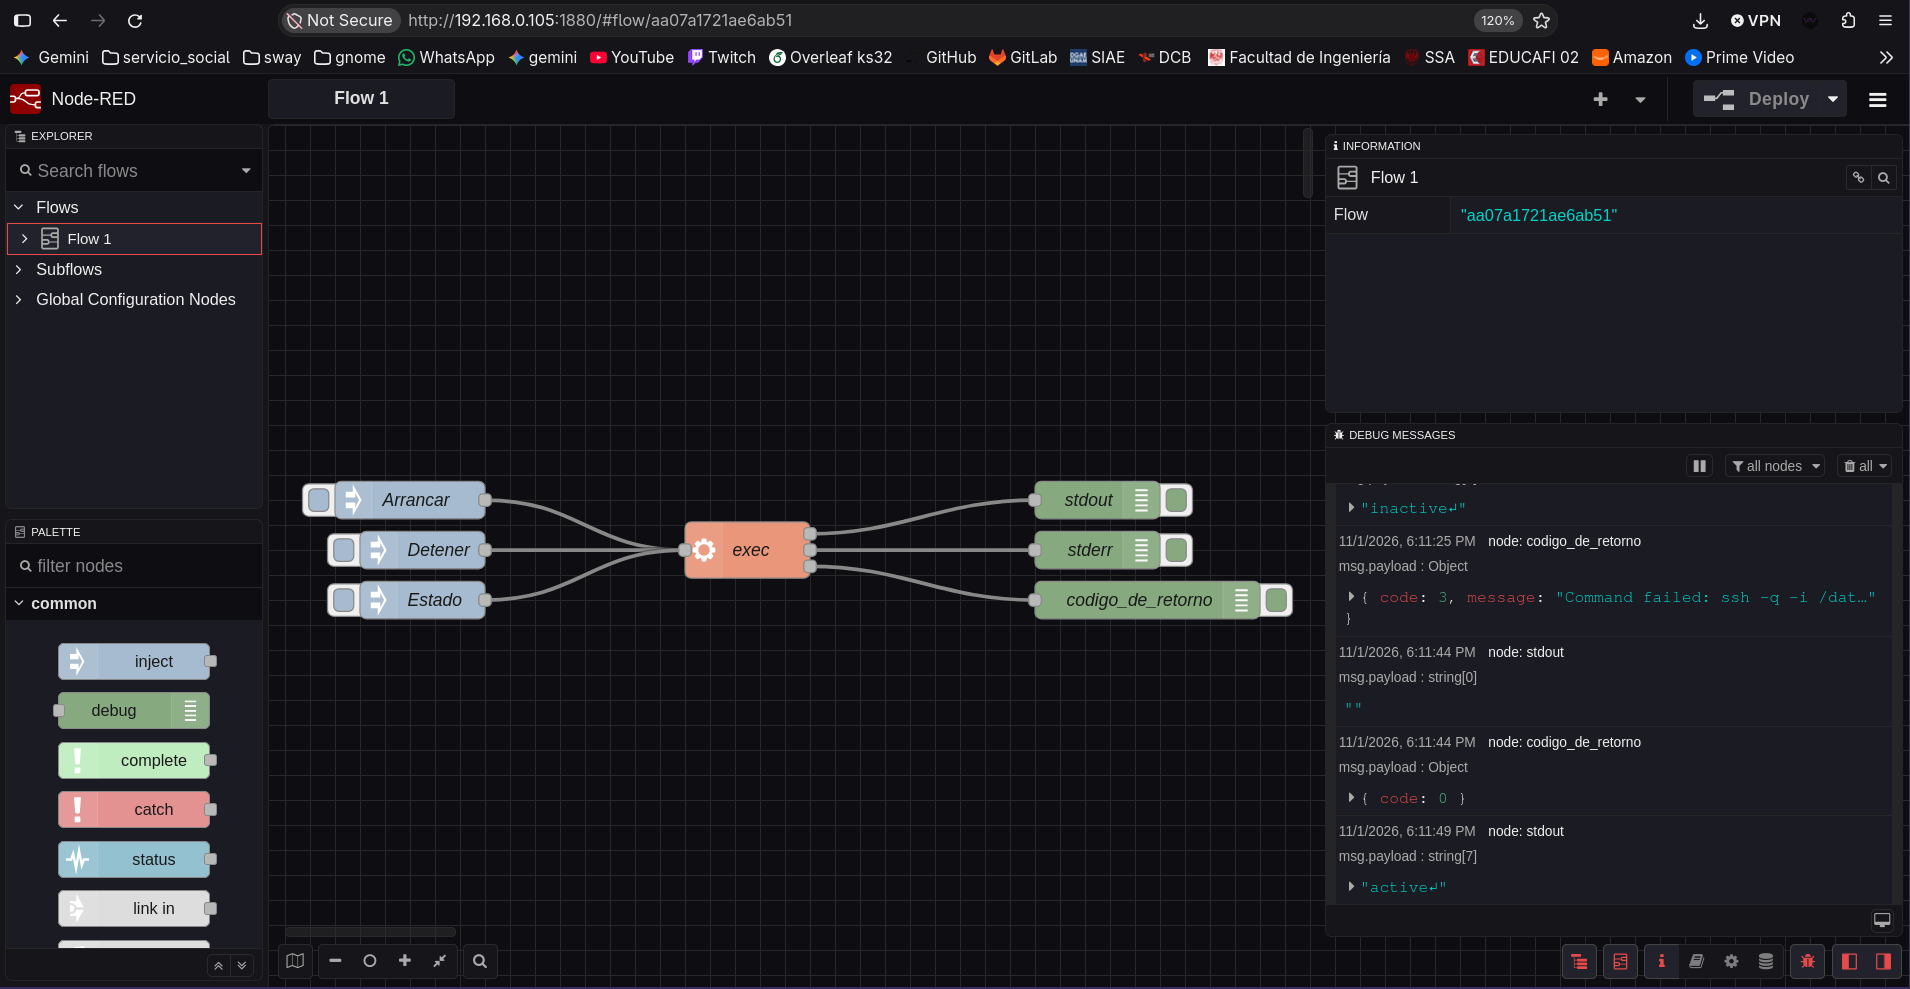
\includegraphics[width=\textwidth]{nodered_debug_message.png}
    \caption{Panel debug mostrando las respuestas de \texttt{systemctl} ante los comandos inyectados.}
    \label{fig:panel_debug}
\end{figure}

Esta implementación final subraya el valor de la programación \textit{low-code} en entornos IoT. Al encapsular la complejidad de las conexiones SSH y las llamadas al sistema en bloques visuales preconfigurados, se reduce significativamente la fricción operativa. Aunque el desarrollo inicial requiere conocimientos técnicos para configurar las llaves y contenedores, una vez establecido, permite que operadores sin experiencia profunda en administración de sistemas Linux puedan integrar, monitorear y controlar el hardware mediante interfaces gráficas intuitivas.

\section*{\centering \fontsize{14}{17}\sffamily\selectfont Conclusiones}

Después de hacer esta práctica, queda clara la diferencia entre controlar servicios con Node-RED y hacerlo con programación tradicional (como armar un script en Python o Bash). Armar la lógica en Node-RED fue mucho más rápido y visual, ya que ver los bloques te permite entender todo el flujo de datos a simple vista. En cambio, hacerlo de forma tradicional nos habría obligado a escribir todo el código para manejar la conexión SSH, capturar los errores y procesar los comandos a mano. Curiosamente, lo que más tiempo nos tomó no fue armar el flujo en sí, sino toda la configuración inicial de permisos y llaves.

Por otro lado, aunque el flujo es totalmente visual, el hecho de tener que usar la terminal para instalar Docker, generar las llaves SSH y preparar \texttt{systemd} nos dice mucho sobre los límites del \textit{low-code}. Estas herramientas son una maravilla para conectar sistemas, sensores y hardware de forma rápida, pero siguen dependiendo por completo de que el sistema operativo esté bien configurado. En resumen: el \textit{low-code} te ahorra escribir la lógica de la aplicación, pero no te salva de tener que saber usar Linux.

Yo usaría Node-RED principalmente en proyectos de IoT, automatización de hardware o cuando se necesita sacar un prototipo rápido; sobre todo si en el equipo hay personas de otras áreas (como mantenimiento u operaciones) que necesitan entender o modificar el sistema sin ser expertos en código. Preferiría la programación tradicional para proyectos que exijan mucho rendimiento, donde sea clave llevar un control de versiones estricto con Git (ya que manejar versiones de texto es más fácil que rastrear cambios en los archivos de Node-RED) o en sistemas muy grandes que dependan de pruebas automatizadas.

% \section{Bibliografía}

\begin{biblio}
	% for: https://sistemasmultibasededatos.blogspot.com/
	\item Esquivel Martinez H. (2021, Noviembre 28). \textit{SISTEMAS MULTIBASE DE DATOS} [Online]. Disponible en: \newline \textcolor{blue}{\underline{\url{https://sistemasmultibasededatos.blogspot.com/}}}
\end{biblio}

\end{document}
